\documentclass[12pt,twoside]{article}
\usepackage[dvipsnames]{xcolor}
\usepackage{tikz,graphicx,amsmath,amsfonts,amscd,amssymb,bm,cite,epsfig,epsf,url}
\usepackage[hang,flushmargin]{footmisc}
\usepackage[colorlinks=true,urlcolor=blue,citecolor=blue]{hyperref}
\usepackage{amsthm,multirow,wasysym,appendix}
\usepackage{array,subcaption} 
% \usepackage[small,bf]{caption}
\usepackage{bbm}
\usepackage{pgfplots}
\usetikzlibrary{spy}
\usepgfplotslibrary{external}
\usepgfplotslibrary{fillbetween}
\usetikzlibrary{arrows,automata}
\usepackage{thmtools}
\usepackage{blkarray} 
\usepackage{textcomp}

\usepackage[left=0.8in,right=1.0in,top=1.0in,bottom=1.0in]{geometry}
\newcommand{\red}[1]{{\leavevmode\color{red}{#1}}}
\newcommand{\blue}[1]{{\leavevmode\color{blue}{#1}}}
\usepackage{graphicx}
%% Probability operators and functions
%
% \def \P{\mathrm{P}}
\def \P{\mathrm{P}}
\def \E{\mathrm{E}}
\def \Var{\mathrm{Var}}
\let\var\Var
\def \Cov {\mathrm{Cov}} \let\cov\Cov
\def \MSE {\mathrm{MSE}} \let\mse\MSE
\def \sgn {\mathrm{sgn}}
\def \R {\mathbb{R}}
\def \C {\mathbb{C}}
\def \N {\mathbb{N}}
\def \Z {\mathbb{Z}}
\def \cV {\mathcal{V}}
\def \cS {\mathcal{S}}

\newcommand{\RR}{\ensuremath{\mathbb{R}}}

\DeclareMathOperator*{\argmin}{arg\,min}
\DeclareMathOperator*{\argmax}{arg\,max}
\newcommand{\red}[1]{\textcolor{red}{#1}}
\newcommand{\blue}[1]{\textcolor{blue}{#1}}
\newcommand{\green}[1]{\textcolor{ForestGreen}{ #1}}
\newcommand{\fuchsia}[1]{\textcolor{RoyalPurple}{ #1}}

\newcommand{\wrnd}[1]{\widetilde{ #1 } }
\newcommand{\po}{\wrnd{\op{po}}  }

%
%% Probability distributions
%
%\def \Bern    {\mathrm{Bern}}
%\def \Binom   {\mathrm{Binom}}
%\def \Exp     {\mathrm{Exp}}
%\def \Geom    {\mathrm{Geom}}
% \def \Norm    {\mathcal{N}}
%\def \Poisson {\mathrm{Poisson}}
%\def \Unif    {\mathrm {U}}
%
\DeclareMathOperator{\Norm}{\mathcal{N}}

\newcommand{\bdb}[1]{\textcolor{red}{#1}}

\newcommand{\ml}[1]{\mathcal{ #1 } }
\newcommand{\wh}[1]{\widehat{ #1 } }
\newcommand{\wt}[1]{\widetilde{ #1 } }
\newcommand{\conj}[1]{\overline{ #1 } }
\newcommand{\rnd}[1]{\tilde{ #1 } }
\newcommand{\rv}[1]{ \rnd{ #1}  }
\newcommand{\rM}{\rnd{ m}  }
\newcommand{\rx}{\rnd{ x}  }
\newcommand{\ry}{\rnd{ y}  }
\newcommand{\rz}{\rnd{ z}  }
\newcommand{\ra}{\rnd{ a}  }
\newcommand{\rb}{\rnd{ b}  }
\newcommand{\rt}{\rnd{ t}  }
\newcommand{\rs}{\rnd{ s}  }


\newcommand{\rpc}{\widetilde{ pc}  }
\newcommand{\rndvec}[1]{\vec{\rnd{#1}}}

\def \cnd {\, | \,}
\def \Id { I }
\def \J {\mathbf{1}\mathbf{1}^T}

\newcommand{\op}[1]{\operatorname{#1}}
\newcommand{\setdef}[2]{ := \keys{ #1 \; | \; #2 } }
\newcommand{\set}[2]{ \keys{ #1 \; | \; #2 } }
\newcommand{\sign}[1]{\op{sign}\left( #1 \right) }
\newcommand{\trace}[1]{\op{tr}\left( #1 \right) }
\newcommand{\tr}[1]{\op{tr}\left( #1 \right) }
\newcommand{\inv}[1]{\left( #1 \right)^{-1} }
\newcommand{\abs}[1]{\left| #1 \right|}
\newcommand{\sabs}[1]{| #1 |}
\newcommand{\keys}[1]{\left\{ #1 \right\}}
\newcommand{\sqbr}[1]{\left[ #1 \right]}
\newcommand{\sbrac}[1]{ ( #1 ) }
\newcommand{\brac}[1]{\left( #1 \right) }
\newcommand{\bbrac}[1]{\big( #1 \big) }
\newcommand{\Bbrac}[1]{\Big( #1 \Big)}
\newcommand{\BBbrac}[1]{\BIG( #1 \Big)}
\newcommand{\MAT}[1]{\begin{bmatrix} #1 \end{bmatrix}}
\newcommand{\sMAT}[1]{\left(\begin{smallmatrix} #1 \end{smallmatrix}\right)}
\newcommand{\sMATn}[1]{\begin{smallmatrix} #1 \end{smallmatrix}}
\newcommand{\PROD}[2]{\left \langle #1, #2\right \rangle}
\newcommand{\PRODs}[2]{\langle #1, #2 \rangle}
\newcommand{\der}[2]{\frac{\text{d}#2}{\text{d}#1}}
\newcommand{\pder}[2]{\frac{\partial#2}{\partial#1}}
\newcommand{\derTwo}[2]{\frac{\text{d}^2#2}{\text{d}#1^2}}
\newcommand{\ceil}[1]{\lceil #1 \rceil}
\newcommand{\Imag}[1]{\op{Im}\brac{ #1 }}
\newcommand{\Real}[1]{\op{Re}\brac{ #1 }}
\newcommand{\norm}[1]{\left|\left| #1 \right|\right| }
\newcommand{\norms}[1]{ \| #1 \|  }
\newcommand{\normProd}[1]{\left|\left| #1 \right|\right| _{\PROD{\cdot}{\cdot}} }
\newcommand{\normTwo}[1]{\left|\left| #1 \right|\right| _{2} }
\newcommand{\normTwos}[1]{ \| #1  \| _{2} }
\newcommand{\normZero}[1]{\left|\left| #1 \right|\right| _{0} }
\newcommand{\normTV}[1]{\left|\left| #1 \right|\right|  _{ \op{TV}  } }% _{\op{c} \ell_1} }
\newcommand{\normOne}[1]{\left|\left| #1 \right|\right| _{1} }
\newcommand{\normOnes}[1]{\| #1 \| _{1} }
\newcommand{\normOneTwo}[1]{\left|\left| #1 \right|\right| _{1,2} }
\newcommand{\normF}[1]{\left|\left| #1 \right|\right| _{\op{F}} }
\newcommand{\normLTwo}[1]{\left|\left| #1 \right|\right| _{\ml{L}_2} }
\newcommand{\normNuc}[1]{\left|\left| #1 \right|\right| _{\ast} }
\newcommand{\normOp}[1]{\left|\left| #1 \right|\right|  }
\newcommand{\normInf}[1]{\left|\left| #1 \right|\right| _{\infty}  }
\newcommand{\proj}[1]{\mathcal{P}_{#1} \, }
\newcommand{\diff}[1]{ \, \text{d}#1 }
\newcommand{\vc}[1]{\boldsymbol{\vec{#1}}}
\newcommand{\rc}[1]{\boldsymbol{#1}}
\newcommand{\vx}{\vec{x}}
\newcommand{\vy}{\vec{y}}
\newcommand{\vz}{\vec{z}}
\newcommand{\vu}{\vec{u}}
\newcommand{\vv}{\vec{v}}
\newcommand{\vb}{\vec{\beta}}
\newcommand{\va}{\vec{\alpha}}
\newcommand{\vaa}{\vec{a}}
\newcommand{\vbb}{\vec{b}}
\newcommand{\vg}{\vec{g}}
\newcommand{\vw}{\vec{w}}
\newcommand{\vh}{\vec{h}}
\newcommand{\vbeta}{\vec{\beta}}
\newcommand{\valpha}{\vec{\alpha}}
\newcommand{\vgamma}{\vec{\gamma}}
\newcommand{\veta}{\vec{\eta}}
\newcommand{\vnu}{\vec{\nu}}
\newcommand{\rw}{\rnd{w}}
\newcommand{\rvnu}{\vc{\nu}}
\newcommand{\rvv}{\rndvec{v}}
\newcommand{\rvw}{\rndvec{w}}
\newcommand{\rvx}{\rndvec{x}}
\newcommand{\rvy}{\rndvec{y}}
\newcommand{\rvz}{\rndvec{z}}
\newcommand{\rvX}{\rndvec{X}}


\newtheorem{theorem}{Theorem}[section]
% \declaretheorem[style=plain,qed=$\square$]{theorem}
\newtheorem{corollary}[theorem]{Corollary}
\newtheorem{definition}[theorem]{Definition}
\newtheorem{lemma}[theorem]{Lemma}
\newtheorem{remark}[theorem]{Remark}
\newtheorem{algorithm}[theorem]{Algorithm}

% \theoremstyle{definition}
%\newtheorem{example}[proof]{Example}
\declaretheorem[style=definition,qed=$\triangle$,sibling=definition]{example}
\declaretheorem[style=definition,qed=$\bigcirc$,sibling=definition]{application}

%
%% Typographic tweaks and miscellaneous
%\newcommand{\sfrac}[2]{\mbox{\small$\displaystyle\frac{#1}{#2}$}}
%\newcommand{\suchthat}{\kern0.1em{:}\kern0.3em}
%\newcommand{\qqquad}{\kern3em}
%\newcommand{\cond}{\,|\,}
%\def\Matlab{\textsc{Matlab}}
%\newcommand{\displayskip}[1]{\abovedisplayskip #1\belowdisplayskip #1}
%\newcommand{\term}[1]{\emph{#1}}
%\renewcommand{\implies}{\;\Rightarrow\;}



\begin{document}

\begin{center}
{\large{\textbf{Homework 3}} } \vspace{0.2cm}\\
Due October 2 at 11 pm
\\
\end{center}
Unless stated otherwise, justify any answers you give.
You can work in groups, but each
student must write their own solution based on their own
understanding of the problem.

When uploading your homework to Gradescope you will have to
select the relevant pages for each question.  Please submit each
problem on a separate page (i.e., 1a and~1b can be on the same page but 1
and 2 must be on different pages).  We understand that this may be
cumbersome but this is the best way for the grading team to grade your
homework assignments and provide feedback in a timely manner.  Failure
to adhere to these guidelines may result in a loss of points.
Note that it may take some time to
select the pages for your submission.  Please plan accordingly.  We
suggest uploading your assignment at least 30 minutes before the deadline
so you will have ample time to select the correct pages for your
submission.  If you are using \LaTeX, consider using the minted or
listings packages for typesetting code.  
\\

\begin{enumerate}

\item (Fish)
A biologist is studying a rare species of fish. She captures four individuals and measures their weights, which are 5, 8, 5 and 6 kg.
\begin{enumerate}
\item
What is the empirical conditional probability that a fish weighs more than 7 kg given that they weigh more than 6 kg? 
\blue{
\begin{itemize}
    \item we could solve for P(fish weighs more than 7k given it weighs more than 6kg) as $\frac{\text{ weigh More than 7kg and weigh more than 6kg}}{\text{ weigh more than 6 kg}}=\frac{1}{1}=1$ so there is a 100$\%$ according to the empirical estimate
\end{itemize}
}

\item Plot an estimate of the pdf of the fish weight using kernel density estimation with a rectangular kernel of width 2. plot the bins as discrete .
\blue{
\begin{itemize}
  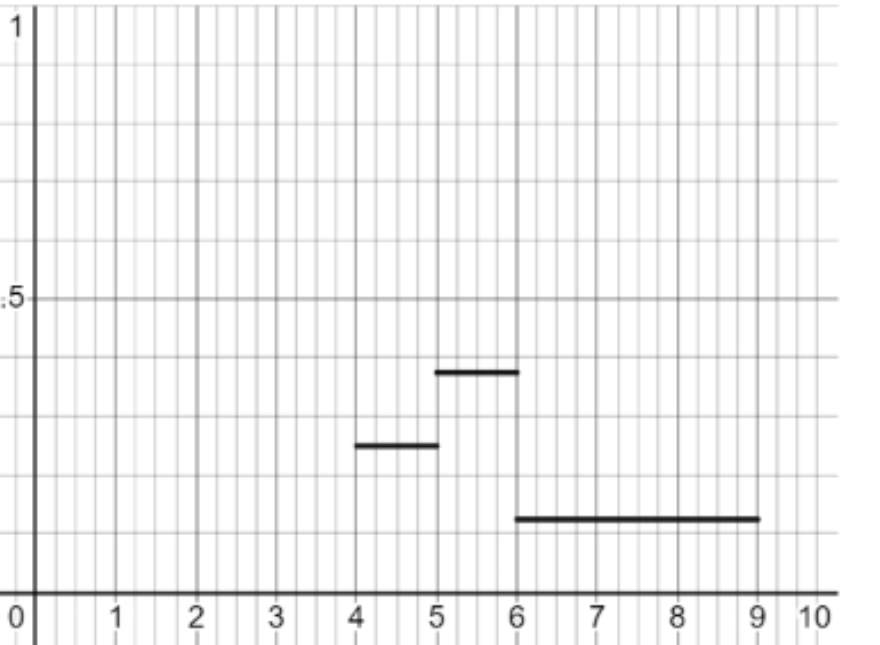
\includegraphics[width=15cm]{homework 3/temp 2 .png}
\end{itemize}
}
\item What is the conditional probability that a fish weighs more than 7 kg given that they weigh more than 6 kg according to your estimated pdf?
\end{enumerate}
\blue{
\begin{itemize}
    \item again we have $\frac{\text{ weigh More than 7kg and weigh more than 6kg}}{\text{ weigh more than 6 kg}}=\frac{\text{ weigh More than 7kg}}{\text{ weigh more than 6 kg}}$
    \item if we look at the area of fish that weigh more than 7, we can see it is 
    \frac{2}{8}
    \item if we look at the area of the pdf greater than 6 we can see that the area is \frac{3}{87}
    \item thus the ratio is $\frac{2}{3}$
    \item note that here i used area calculations instead of integrating as our pdf in this case is not continuous 
\end{itemize}}
\newpage

\item (Nuclear power plant)
The random variable $\rt$ with the following pdf
\begin{figure}[h]
\begin{center}
\begin{tikzpicture}
\begin{axis}[xmin= -2, xmax=5, ymin=-0.1, ymax=0.7, xlabel=$t$,
ylabel=$f_{\rt}(t)$,height=4cm,
width=0.7\textwidth,
xticklabels={-1,0,...,4}, xtick={-1,0,1,...,4},
yticklabels={0,$\alpha$}, ytick={0,0.5}]
%\addplot+[ycomb, blue, very thick, samples=2] coordinates {(0,1)(1,1)};
\addplot[blue, very thick, samples=2] coordinates {(-2,0)(-1,0)};
\addplot[blue, very thick, samples=2] coordinates {(-1,0.5)(0,0.5)};
%\addplot[dashed,blue, very thick, samples=2] coordinates {(0,0)(0,0.5)};
\addplot[dashed, blue, very thick, samples=2] coordinates {(-1,0)(-1,0.5)};
\addplot[blue, very thick, domain=0:6, samples=101] {0.5*exp(-x)};
\node at (axis cs:1,0.3) [anchor=south west] {$\alpha e^{-t}$};
%\addplot[dashed,blue, very thick, samples=2] coordinates {(0,0)(0,0.5)};
\end{axis}
\end{tikzpicture} 
\end{center}
\end{figure}\\
models the time at which there is a leak in a nuclear power plant. The pdf is constant during the time the station is built (between -1 and 0) and exponential with parameter 1 afterwards (from 0 to $+\infty$). 
\begin{enumerate}
\item Compute the value of the constant $\alpha$. 
\blue{
\begin{itemize}
    \item for this PDF to make sense it must be the case that $\int_{-1}^{0}\alpha dt+\int_{0}^{\infty}\alpha e^{-t} dt=1$ 
    \item we can see that $\int_{-1}^{0}\alpha dt+\int_{0}^{\infty}\alpha e^{-t} dt=\alpha|_{-1}^{0}-\alpha e^{-t}|_{0}^{\infty}=2\alpha$
    \item thus it must be the case that $2\alpha=1$ meanign that $\alpha=\frac{1}{2}$
\end{itemize}}
\item Compute the cdf of $\rt$ and plot it.
\blue{
\begin{itemize}
    \item the cdf is $F_\Tilde{T}(t)=P(\Tilde{t}\leq t)$
    \item if $t\leq -1$ $F_\Tilde{T}(t)=0$
    \item if $t\leq 0 and t\geq -1$ we know $F_\Tilde{T}(t)=\int_{-1}^{t}\frac{1}{2}du=\frac{1}{2}u|_{-1}^{t}=\frac{1+t}{2}$
    \item if $t \geq 0$ it must be the case that$F_\Tilde{T}(t)=\int_{-1}^{t}\frac{1}{2}du+\int_{0}^{\infty}\frac{1}{2}e^{-u}du=\frac{1}{2}|_{-1}^{0}+\frac{-1}{2}e^{-u}|_{0}^{t}=\frac{1}{2}-\frac{1}{2}e^{-u}|_{0}^{t}\\=1-\frac{1}{2}e^{-t}$
    \item so finally we see that $f_{\Tilde{t}}(t) = 
\left\{
    \begin{array}{lr}
        0, & \text{if } t \leq -1\\
        \frac{1+t}{2}, & \text{if } t\leq 0 \text{ and } t\geq -1\\
        1-\frac{1}{2}e^{-t}&  \text{ if } t\geq 0
        
    \end{array}$
    
    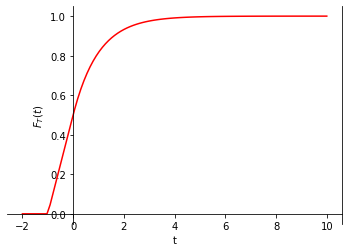
\includegraphics[width=15cm]{homework 3/question 2.png}
\end{itemize}
}

\item Compute the pdf of $\rt$ conditioned on $\rt <0$.
\blue{
\begin{itemize}
    \item first let us solve for the new cdf. 
    \item so we know we are looking for the likclyhood that $\Tilde{t}>y$ given t is less than 0 this can be expressed as $P(\Tilde{t}<y|\Tilde{y}<0)=\frac{P(\Tilde{t}<y \cap \Tilde{t}<0)}{P(\Tilde{t}<0)}=\frac{1-P(\Tilde{t}>y \cap \Tilde{t}<0)}{P(\Tilde{t}<0)}$ \item this can be expressed in terms of the cdf we already know as 
    $\frac{1-P(\Tilde{t}>y \cap \Tilde{t}<0)}{P(\Tilde{t}<0)}=\frac{1-(F_{\Tilde{t}}(0)-F_{\Tilde{t}}(y))}{F_{\Tilde{t}}(0)}=\frac{1-\frac{1}{2}+\frac{1+y}{2}}{\frac{1}{2}}=\frac{\frac{1}{2}+\frac{1+y}{2}}{\frac{1}{2}}=1+\frac{2(1+y)}{2}=2+y$ 
    \item we can call this new cdf $G_{\Tilde{t}}(y) = 
\left\{
    \begin{array}{lr}
        2+y, & \text{if } y\leq 0 \text{ and } y\geq -1\\
        0&  \text{otherwise }
    \end{array}$
    \item then we know that the pdf we are looking for is the darivative of this cdf so we can see that $g_{\Tilde{t}}(y)=\frac{dG_{\Tilde{t}(y)}}{dy}=\left\{
    \begin{array}{lr}
        1, & \text{if } y\leq 0 \text{ and } y\geq -1\\
        0&  \text{otherwise }
    \end{array}$
    \item then we can check that this is sensible as $\int_{\mathbb{R}}g{\Tilde{t}}(y)dy=\int_{-\infty}^{-1}0dy+\int_{-1}^{0}1dy+\int_{0}^{\infty}0dy=1$
    
\end{itemize}

}
\end{enumerate}
\newpage
\item (Measurements)  
You have access to the readings of a device that indicates whether a radioactive particle has decayed. However you do not get a continuous reading, you get a reading every second. 
\begin{enumerate}
\item A reasonable model for the time the particle takes to decay is that it is a random variable with pdf
\begin{align}
f_{\rnd{t}}(t) := \begin{cases}
$\lambda \exp(- \lambda t), \qquad \text{if $t\geq 0$},\\
0$ \qquad \text{otherwise},
\end{cases}
\end{align}
where $\lambda$ is a fixed constant. Taking into account that the measurement device rounds up the time and outputs an integer number of seconds (if the time is $0.1$ it outputs 1, if it is 13.4 it outputs 14), compute the pmf of the reading from the device. What kind of random variable is this? 
\blue{
\begin{itemize}
    \item let int(a) be the function that rounds the real numebr a up to the nearest integer
    \item we can see that $P(\Tilde{t}=x)=\int_{int(x-1)}^{int(x)}\lambda e^{-\lambda t}dt=-e^{-\lambda t}|_{int(x-1)}^{int(x)}\\=e^{-\lambda(int(x-1))}-e^{-\lambda(int(x))}$
    if $t\geq 0$ and 0 elsewhere
    \item this is gemoetric distrobutin 
    \item F_{\rnd{t}}(t) := \begin{cases}
$(1-e^{-\lambda})e^{-\lambda(t-1)}, \qquad \text{if $t\geq 0$},\\
0$ \qquad \text{otherwise},
\end{cases}
\end{itemize}
}
\item What is the pdf of the error between your reading and the true time of decay?
\blue{
\begin{itemize}
\item we must first deffine a few things.
\item \Tilde{R} be the random varible represneting the possible outcomes for the actual time decay 
\item let \Tilde{t} be the random varible represening our measurment 
\item let \Tilde{e}=\Tilde{t}-\Tilde{r} be the random varible represting the error
\item we can see that the cdf of the error is 
\item $F_\Tilde{e}(t)=P(\Tilde{e}\leq e)=P(\Tilde{t}-\Tilde{r}\leq e)$ we know that r can take on values between 1 and infinty units of time. so we can express this using a union of sets $P(\Tilde{t}-\Tilde{r}\leq e)=P(U_{r=1}^{\infty}\{\r-r\leq \Tilde{t}\leq r\})$ so we are looking at the the union of the liclyhood that t is in many disjoint intervals 
\item so we can express this as a sum of proabilit.es
\item that is $P(U_{r=1}^{\infty}\{r-e\leq \Tilde{t}\leq r\})=\sum_{r=1}^{\infty}P(r-e\leq \Tilde{t}\leq r)=\sum_{r=1}^{\infty}\int_{t-e}^tf\Tilde{t}(t)dt=\sum_{r=1}^{\infty}\int_{t-e}^t(1-e^{-\lambda})e^{-\lambda(t-1)}dt=\sum_{r=1}^{\infty}(e^-\lambda r)(e^{\lambda x}-1)=\frac{e^{\lambda y}-1}{e^{\lambda}-1}$
\item so finalyl we see that our Cdf is $F\Tilde{e}=\frac{e^{\lambda y}-1}{e^{\lambda}-1}$ if t is betwene 0 and 1 and 0 elsewhere 
\item so taking the davivative of the cdf we can see that the pdf is $f_t(t)=\frac{\lambda e^{\lambda t}}{e^{\lambda}-1 }$ if t is between 0 and 1 and 0 elsewhere 
\end{itemize}
}
\end{enumerate}
\newpage
\item (Applying the cdf) The array in \texttt{samples.npy} contains $n := 1,000$ i.i.d. samples from a certain distribution. 
\begin{enumerate}
\item Compute the empirical cdf of the data $F_X$ and plot it.
\blue{
\begin{itemize}
    \item 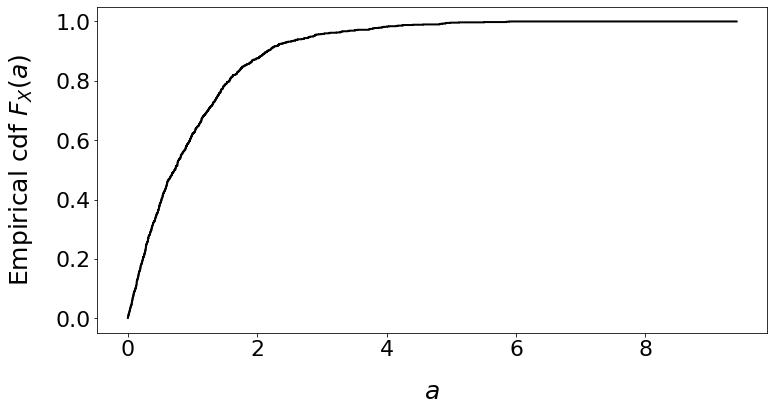
\includegraphics[width=15cm]{homework 3/empircal question 3.png}
\end{itemize}
}

\item If you apply the empirical cdf to each data point $x_i$ , $1\leq i \leq n$, to obtain a new data point $y_i := F_X(x_i)$, what are the new data equal to? Does your answer depend on the distribution of the data?
\blue{
\begin{itemize}
    \item by theorem 3.23 we know that $y_i$ will be uniformly distributed regardless of the distribution of the data.
\end{itemize}


}
\end{enumerate}
\end{enumerate}
\end{document}
